\section{Auswertung}
\label{sec:Auswertung}
Bei dem beschriebenen Messverfahren wurden die im Anhang befindlichen Messkurven mit einem x-y-Schreiber aufgenommen.
Aus diesen kann, mittels einer Messskala $\xi$, die Lage des jeweiligen Resonanzminimums bestimmt werden. Aus der willkürlichen Messskala ergeben sich Fehler beim Ablesen und Umrechnen. Diese werden in den weiteren Rechnungen mittels Gaußscher Fehlerfortpflanzung berücksichtigt.

\begin{table}[h]
\centering
\caption{CAPTION}
\sisetup{%uncertainty-seperator = {\,},
table-number-alignment = center,
table-unit-alignment = center,
%table-figures-integer = 1,
%table-figures-decimal = 1,
table-auto-round = true
}
\begin{tabular}{ S[table-format= 3.1]
 @{\,$\pm{}$\,} 
 S[table-format= 3.1] S[table-format= 3.1]
 @{\,$\pm{}$\,} 
 S[table-format= 3.1] S[table-format= 3.1]
 @{\,$\pm{}$\,} 
 S[table-format= 3.1] S[table-format= 3.1]
 @{\,$\pm{}$\,} 
 S[table-format= 3.1] S[table-format= 3.1]
 @{\,$\pm{}$\,} 
 S[table-format= 3.1] S[table-format= 3.1]
 @{\,$\pm{}$\,} 
 S[table-format= 3.1]  S[table-format= 3.1] 
}
\toprule
\multicolumn{2}{c}{TITLE}
&\multicolumn{2}{c}{TITLE}
&\multicolumn{2}{c}{TITLE}
&\multicolumn{2}{c}{TITLE}
&\multicolumn{2}{c}{TITLE}
&\multicolumn{2}{c}{TITLE}
&{$\text{Title}$} \\
 \midrule
1.831611815552305&0.050481183020468&218.90703803982444&2.725983883105272&308.6560170018874&5.1995618511082045&0.30706418706675404&0.0038237784975671454&0.43295642658462413&0.007293503430544743&0.3700103068256891&0.005558640964055944&10.572\\
1.8975486746422707&0.05726387650505347&352.7504691531785&3.493096466808262&419.164672765658&5.497332144485133&0.4948083762762867&0.004899818829630765&0.5879685762614596&0.007711190289254972&0.5413884762688731&0.006305504559442869&15.901\\
1.84252360689672&0.07313277976918699&477.15002593794907&7.825207435303008&545.3233993931276&10.531120286762928&0.6693055012551137&0.010976535890604409&0.7649333151758535&0.014772160450906867&0.7171194082154836&0.012874348170755636&20.557\\
1.8721371882086169&0.06274502065668285&598.8854875283447&2.509800826267314&668.1545634920635&4.8313665905645795&0.840065659928726&0.0035205352798069337&0.9372304321997529&0.006777030413628347&0.8886480460642393&0.00514878284671764&25.0\\
1.7939749567538612&0.08968960282489664&704.8697961943399&7.892685048590905&769.4528946374788&11.121510750287184&0.9887314400414475&0.011071187751298277&1.0793231213289487&0.015600310013193026&1.034027280685198&0.013335748882245651&29.448\\
\bottomrule
\end{tabular}
\label{tab:LABEL}
\end{table}

Da das Verfahren auf sehr kleinen Magnetfeldern beruht, muss das Erdmagnetfeld als Störfaktor unbedingt berücksichtigt werden. Aus den, zum Magnetfeld, parallelen und antiparallelen Messungen, werden die Ströme abgelesen. Aus diesen kann mit

Spulenhalbmesser $r = \SI{0.1}{\meter}$
Windungszahl $n = 156$

\begin{equation}
    B(I)= \frac{8}{\sqrt{125}}\mu_0\frac{n}{r}I
\end{equation}

das Magnetfeld $B$ der Helmholtzspule berücksichtigt werden.
Die Messwerte des Stroms und die berechneten Magnetfelder, sowie die Messskala $\xi$ finden sich in Tabelle \ref{tab:tab}.
Dabei bedeuten die mit $a$ und $p$ indizierten Größen, die jeweilige antiparallele oder parallele Messung. Der Mittelwert aus diesen ist das wahre Magnetfeld $\bar B$. 
Als Nebenprodukt kann mit diesen Werten das Erdmagnetfeld bestimmt werden.
Dies ergibt
\begin{equation}
	B_\text{Erde} = \frac{B_p - B_a}{2} = \SI{50.2\pm 0.08}{\micro\tesla}
\end{equation}
als Mittelwert.
Nach \eqref{eqn:B} hängen $B$ und $\Delta E$ linear voneinander ab.
Umstellen ergibt
\begin{equation}
	B = \frac{h}{\mu_B g} \nu
\end{equation}
für das Magnetfeld.
Daraus ist ersichtlich, dass die gesuchte Größe $g$, das gyromagnetische Verhältnis des Elektrons, aus einer linearen Regressionsrechnung bestimmt werden kann.
Nach
\begin{equation}
	B = m\cdot\nu + b
\end{equation}
lassen sich die Fitparameter $m$ und $b$ bestimmen. Der y-Achsnabschnitt liegt bei etwa $b = -4{,}86\cdot10^{-6}$, was einer zu erwartenden Ursprungsgerade sehr nahe kommt.
Aus dem Parameter $m$ kann das gyromagnetische Verhältnis zu
\begin{equation}
	g = \frac{h}{\mu_B m} = \SI{2.025\pm0.024}{}
\end{equation} 
bestimmt werden.
In Abbildung \ref{fig:plot} sind die eingetragenen Messwerte und die Regressionsgerade zu sehen.



\begin{figure}
	\centering
	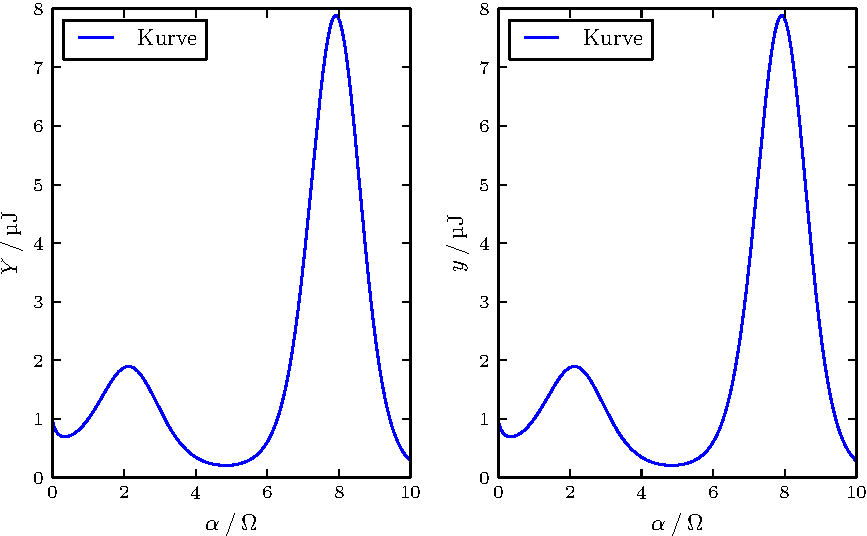
\includegraphics[]{pc/plot.pdf}
	\caption{Hier sind Methwerte und eine Rezessionsgerade.}
	\label{fig:plot}
\end{figure}
